\documentclass[12pt, twoside]{article}
\usepackage[a4paper, margin=0.9in]{geometry}
\usepackage{polski}
\usepackage[utf8]{inputenc}
\usepackage{graphicx}
\usepackage{xcolor,listings}
\usepackage{float}
\usepackage{minted}
\usepackage{rotating}
\usepackage{fancyhdr}
\usepackage{array}
\usepackage{amsmath}
\newcolumntype{M}{>{\centering\let\newline\\\arraybackslash\hspace{0pt}}m{2.5cm}}
\fancyhf{} % clear all header and footers
\renewcommand{\headrulewidth}{0pt} % remove the header rule
\fancyfoot[LE,RO]{\thepage} % Left side on Even pages; Right side on Odd pages
\pagestyle{fancy}
\fancypagestyle{plain}{%
    \fancyhf{}%
    \renewcommand{\headrulewidth}{0pt}%
    \fancyhf[lef,rof]{\thepage}%
}

\usepackage{hyperref}
\hypersetup{
    colorlinks,
    citecolor=black,
    filecolor=black,
    linkcolor=black,
    urlcolor=black
}

\begin{document}

\title{\vspace{50mm}Problem ośmiu hetmanów \\
    \large Sztuczna Inteligencja - Projekt  
}

\author{Dawid Paluch}
\date{\today}
\maketitle

\begin{center}
    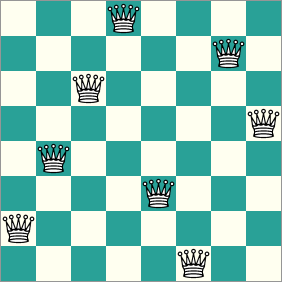
\includegraphics[keepaspectratio=true, scale=0.6]{8queens.png}
\end{center}
\thispagestyle{empty}
\clearpage
\setcounter{page}{1}

\clearpage
\tableofcontents
\clearpage

\setcounter{page}{3}
\section{Wprowadzenie}

\subsection{Problem ośmiu hetmanów}
W jaki sposób ustawić osiem hetmanów na szachownicy 8x8 by wzajemnie się nie atakowały? Ile jest możliwych ustawień?

\subsection{Historia problemu}
Problem ośmiu hetmanów został po raz pierwszy sformułowany w 1848 roku przez mistrza szachowego Maksa Bezzela (1824-1871). Pierwsze rozwiązanie podał dwa lata później Franz Nauck. Również matematyk Carl Friedrich Gauss interesował się tym problemem. W roku 1992 wskazano na związki pomiędzy problemem ośmiu hetmanów a kwadratami magicznymi.

\subsection{Reprezentacja rozwiązań}
Rozwiązania problemu przedstawiamy za pomocą ośmiu cyfr odpowiadających za kolejne kolumny szachownicy. Każda z cyfr określa wiersz na którym ustawiony jest hetman. Przykładowe rozwiązanie przedstawia rys. \ref{fig:example}.

\begin{figure}[H]
    \centering
    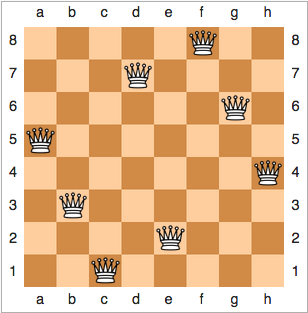
\includegraphics[keepaspectratio=true, scale=0.7]{example-53172864.png}
    \caption{Przykładowe rozwiązanie - 53172864}
    \label{fig:example}
\end{figure}

\clearpage
\section{Algorytm genetyczny}
\subsection{Opis algorytmu}
Problem ośmiu hetmanów możemy rozwiązać za pomocą algorytmu genetycznego. Populacją w naszym algorytmie będzie zbiór ustawień hetmanów. Każdy z osobników charakteryzuje się określonym dopasowaniem - im większe tym bliżej mu do prawidłowego rozwiązania.\\
Maksymalne dopasowanie dla problemu n-hetmanów określone jest wzorem:
\[ f_{max} = \dfrac{n(n - 1)}{2} \]
Co w przypadku problemu ośmiu hetmanów daje nam:
\[ f_{max} = \dfrac{8(8 - 1)}{2} = \dfrac{8 \cdot 7}{2} = 28 \]
Stopień dopasowania obliczymy odejmując liczbę atakujących się hetmanów(nazywaną też liczbą kolizji) od dopasowania maksymalnego:
\[ f = f_{max} - c\]
Osobniki z większym dopasowaniem będą miały większe prawdopodobieństwo reprodukcji, a co za tym idzie będą chętniej wybierane przez algorytm. Prawdopodobieństwo to dane jest wzorem:
\[ P(R) = \dfrac{f}{f_{max}}\]
Osobnik 42625782 będzie charakteryzował się dopasowaniem \( f = 24\) oraz prawdopodobieństwem reprodukcji \( P(R) = 0.857143\).
Po wybraniu dwóch osobników z możliwie najwyższym dopasowaniem następuje ich skrzyżowanie względem losowej kolumny. 
Osobnik może zostać zmutowany z bardzo małym prawdopodobieństwiem np.
\[ P(C) = 0.03 \]
Mutacja osobnika polega na przesunięciu losowego hetmana na losowo wybrany wiersz.
\\[12pt]
Proces reprodukcji i ewentualnej mutacji będzie przebiegał aż do uzyskania w populacji osobnika z dopasowaniem maksymalnym, czyli z poprawnym rozwiązaniem problemu. W przypadku problemu ośmiu hetmanów otrzymamy ustawienie ośmiu hetmanów, które nie atakują się nawzajem.

\clearpage
\subsection{Implementacja w języku Python}
Dokonajmy analizy wszystkich części, z których składa się skrypt. Na samym początku generujemy populację o rozmiarze stu osobników. Następnie algorytm powtarza swoje dziłanie aż do znalezienia poprawnego rozwiązania.
\begin{minted}
[
frame=lines,
framesep=2mm,
baselinestretch=1.2,
fontsize=\footnotesize,
linenos
]
{python}
if __name__ == "__main__":
    population = [random_individual(8) for _ in range(100)]
    generation = 1

    while not maxFitness in [fitness(x) for x in population]:
        print("=== Generation {} ===".format(generation))
        population = genetic_queen(population, fitness)
        print("Maximum fitness = {}".format(max([fitness(n) for n in population])))
        generation += 1

    print("Solved in Generation {}!".format(generation-1))
    for x in population:
        if fitness(x) == maxFitness:
            print_individual(x)
\end{minted}

Sam algorytm zawarty jest w funkcji poniżej. Dla podanej populacji zostaje wygenerowana lista prawdopodobieństw, a w kolejnych krokach następuje reprodukcja i mutacja osobników.
\begin{minted}
[
frame=lines,
framesep=2mm,
baselinestretch=1.2,
fontsize=\footnotesize,
linenos
]
{python}
def genetic_queen(population, fitness):
    mutation_probability = 0.03
    new_population = []
    probabilities = [probability(n, fitness) for n in population]
    for i in range(len(population)):
        x = random_pick(population, probabilities)
        y = random_pick(population, probabilities)
        child = reproduce(x, y)
        if random.random() < mutation_probability:
            child = mutate(child)
        print_individual(child)
        new_population.append(child)
        if fitness(child) == maxFitness: break
    return new_population
\end{minted}
\clearpage
Na szczególną uwagę zasługuje funkcja licząca poziom dopasowania osobnika. Całkowita liczba kolizji to kolizje występujące w wierszach i na przekątnych. Kolizje w kolumnach nie są możliwe ze względu na zapis. Każda cyfra odpowiada za inną kolumnę. O ile znalezienie kolizji w wierszach jest dość proste. Niech P będzie zbiorem ustawień hetmanów:
\[ h = \dfrac{n(n - |P|)}{2} \]
Hetman znajdujący się i-tej kolumnie i q\textsubscript{i}-tym wierszu znajduje się też na (\(i+q_i-1\))-tej lewej przekątnej oraz 
(\(n-1+q_i\))-tej prawej przekątnej. Niech zbiory L\textsubscript{i} i R\textsubscript{i} będą kolejnymi lewymi i prawymi przekątnymi, a Q konkretnym ustawieniem:

\[ \forall q_i \in Q, i \in \langle1, n\rangle: q_i \in L_{i+q_i-1} \land q_i \in R_{n-1+q_i}  \]

Liczba kolizji z lewej i prawej przekątnej zostaje podzielona przez ich długość i wyrażona wzorem:
\[ d = \sum_{i=1}^{2n-1}\dfrac{|L_i| + |R_i|}{n - |i-n|}\]
Ostatecznie całkowitą liczbę kolizji otrzymujemy poprzez sumę kolizji w wierszach i przekątnych:
\[ c = \dfrac{n(n - |P|)}{2} + \sum_{i=1}^{2n-1}\dfrac{|L_i| + |R_i|}{n - |i-n|}\]

\begin{minted}
[
frame=lines,
framesep=2mm,
baselinestretch=1.2,
fontsize=\footnotesize,
linenos
]
{python}
maxFitness = 28
def fitness(individual):
    horizontal_collisions = sum([individual.count(queen)-1 for queen in individual])/2
    diagonal_collisions = 0

    n = len(individual)
    left_diagonal = [0] * 2*n
    right_diagonal = [0] * 2*n
    for i in range(n):
        left_diagonal[i + individual[i] - 1] += 1
        right_diagonal[len(individual) - i + individual[i] - 2] += 1

    diagonal_collisions = 0
    for i in range(2*n-1):
        counter = 0
        if left_diagonal[i] > 1:
            counter += left_diagonal[i]-1
        if right_diagonal[i] > 1:
            counter += right_diagonal[i]-1
        diagonal_collisions += counter / (n-abs(i-n+1))

    return int(maxFitness - (horizontal_collisions + diagonal_collisions))
    
\end{minted}

\clearpage
\section{Podsumowanie}


\end{document}
